%Time-stamp: <2006-10-03 18:11:21 hamada>

\documentclass[a4paper,fleqn]{jarticle}
\usepackage{amsmath}
\usepackage{epsfig}
\usepackage{a4wide}
\usepackage{makeidx}
\usepackage{fancyhdr}
\usepackage{graphicx}
\usepackage{float}
\usepackage{alltt}
\usepackage{times}
\ifx\pdfoutput\undefined
\usepackage[ps2pdf,
            pagebackref=true,
            colorlinks=true,
            linkcolor=blue
           ]{hyperref}
\else
\usepackage[pdftex,
            pagebackref=true,
            colorlinks=true,
            linkcolor=blue
           ]{hyperref}
\fi
\usepackage{doxygen}
\numberwithin{equation}{section}
\numberwithin{figure}{section}

\setlength{\textheight}{232mm}

\makeindex
\setcounter{tocdepth}{1}
%% \setlength{\footrulewidth}{0.4pt}
\begin{document}
\begin{titlepage}
\vspace*{7cm}
\begin{center}
{\Large PROGRAPE-4 $B<h$j07$$@bL@=q(B}\\
\vspace*{1cm}
{\large $B_@ED(B $B9d(B}\\
{\small {\bf hamada@progrape.jp}}\\
\vspace*{0.5cm}
{\small Tue Oct  3 2006 : Tsuyoshi Hamada}\\
{\small Tue Oct  2 2006 : Tsuyoshi Hamada}\\
\end{center}
\end{titlepage}
\pagenumbering{roman}
\tableofcontents
\pagenumbering{arabic}

\clearpage
\section{�Ϥ����}
\label{pci64RegMap}

\begin{Desc}
\item[Author: ]\par
Tsuyoshi Hamada,
Time-stamp: <2006-10-03 00:28:19 hamada>
\end{Desc}

 
�����ʤ���Ѥ��������ΤäƤ����Ƥ����������������������Ƥ��ޤ���

%%%%%%%%%%%%%%%%%%%%%%%%%%%%%%%%%%%%%%%%%%%%%%%%%%%%%%%%%%%%%%%%%%%%%%%%%%%%%%%
%%%%%%%%%%%%%%%%%%%%%%%%%%%%%%%%%%%%%%%%%%%%%%%%%%%%%%%%%%%%%%%%%%%%%%%%%%%%%%%
%\subsection{IFPGA �����֥��å���}
%\begin{figure}[h]
%\begin{minipage}[b]{1.0\linewidth}\centering
%  \centerline{\epsfig{file=fig/ifpga.eps,width=180mm}}
%\end{minipage}
%\caption{IFPGA �����֥��å���}
%\label{fig:pci64RegMap:1}
%\end{figure}


%%%%%%%%%%%%%%%%%%%%%%%%%%%%%%%%%%%%%%%%%%%%%%%%%%%%%%%%%%%%%%%%%%%%%%%%%%%%%%%
%%%%%%%%%%%%%%%%%%%%%%%%%%%%%%%%%%%%%%%%%%%%%%%%%%%%%%%%%%%%%%%%%%%%%%%%%%%%%%%
\subsection{PROGRAPE-4}

PROGRAPE-4�Ȥ������ʤ�̾�ΤǤ���PROGRAPE-4�ϡ�������ѥ��������
���ơ���������³���ƻ��Ѥ���׻��ղåܡ��ɤȸƤФ���Τΰ��Ǥ���
¾�η׻��ղåܡ��ɤȤ��礭�ʰ㤤�Ϸ׻��ѤΥǥХ����˥ե�����ɡ��ץ���
��ޥ֥롦�����ȥ��쥤(Field Programmable Gate Array :FPGA ���եԡ�����
����)���Ѥ��Ƥ��뤳�ȤǤ���FPGA�Ȥ�����������ϩ����¤��˽񤭴����뤳
�Ȥ���ǽ�ʥץ�����ޥ֥�ǥХ����Τ�äȤ⹭���Ȥ��Ƥ����ΤǤ���

\subsection{���ջ��� (�����ˤ�����ĺ�������)}

������(PROGRAPE-4)�򥻥åȥ��åפ���ݤˤϡ��Ƽ��Ÿ��ϴ�������ߤ��Ƥ�
�뤳�Ȥ��ǧ���Ʋ��������ѥ������PCI�Х��������ʤ���³����
�ݤˤϡ�ɬ���ѥ�������Ÿ������֥�򥳥󥻥�Ȥ��鳰���Ƥ����Ȥ��
�äƲ�������


\clearpage
\section{PROGRAPE�ϡ��ɥ������Υ��󥹥ȡ���}
\label{Extsupply}

\begin{Desc}
\item[Author: ]\par
Tsuyoshi Hamada,
Time-stamp: <2006-10-03 18:05:31 hamada>
\end{Desc}

�����ʤΥ��󥹥ȡ���ˤĤ����������ޤ���
�����ʤϥѥ������PCI�Х������夷�ƻ��Ѥ��ޤ���
��\ref{fig:hwinstall}�������ʤ�ѥ�����˥��󥹥ȡ��뤷���ͻҤ򼨤���
����

\begin{figure}[h]
\begin{minipage}[b]{1.0\linewidth}\centering
  \centerline{\epsfig{file=fig/pg4-info-hwinstall,width=180mm}}
\end{minipage}
\caption{�ѥ�����˥��󥹥ȡ��뤷��PROGRAPE-4���ͻ�}
\label{fig:hwinstall}
\end{figure}


���󥹥ȡ����ή��ϼ���(1)��(3)�Τ褦�ˤʤ�ޤ���
\begin{itemize}
\item[(1)] �ѥ�������Ÿ��򺬸��������Ǥ��롥
\item[(2)] �����ʤ�ѥ������PCI���ͥ��������夹�롥
\item[(3)] �����ʤγ��������Ÿ��ѥ��ͥ����˥ѥ��������Ÿ��γ����Ÿ���
��³���롥
\end{itemize}






%------------------------------------------------------------------------------------------------
\subsection{���������Ÿ��ѥ��ͥ���}

�����ʤˤϳ����������Ϥ򶡵뤹�뤿��Υ��ͥ���(���������Ÿ��ѥ��ͥ���)��
����ޤ��������ʤ�ɬ�����Υ��ͥ����˳����Ÿ�����³���Ƥ����Ѳ�����(��\ref{fig:Jumper:extsupply2})��
���������Ÿ����ͥ����˳����Ÿ�����³���ʤ��Ǥ����Ѥ�����硤�����ʤ������ư��ޤ���


\begin{figure}[h]
\begin{minipage}[b]{1.0\linewidth}\centering
  \centerline{\epsfig{file=fig/pg4-info-extsupply,width=180mm}}
\end{minipage}
\caption{���������Ÿ��ѥ��ͥ���}
\label{fig:Jumper:extsupply}
\end{figure}

\begin{figure}[h]
\begin{minipage}[b]{1.0\linewidth}\centering
  \centerline{\epsfig{file=fig/pg4-info-extsupply2,width=180mm}}
\end{minipage}
\caption{���������Ÿ��ѥ��ͥ����˳����Ÿ�����³�����ͻ�}
\label{fig:Jumper:extsupply2}
\end{figure}



\clearpage
\section{��­����}
\label{Trouble}

\begin{Desc}
\item[Author: ]\par
Tsuyoshi Hamada,
Time-stamp: <2006-10-03 18:11:36 hamada>
\end{Desc}

��­����ˤĤ����������ޤ���


\subsection{�����ѡ�������}
 
�вٻ��Υ����ѡ�������򼨤��ޤ���
�����Ѥ�û��(Short)�Ȥϡ������ѥԥ�򥸥��Ѥ�ʤ���碌��
���֤��̣���ޤ��������Ѥ�����(Open)�Ȥϥ����ѥԥ�˥����Ѥ�ʤ��
�碌�ʤ�����(�Ĥޤꤽ�Τޤ�)���̣���ޤ���
�ʤ����вٻ��Υ����Ѥ�PCI�Х���64bit/66MHz���̿�����褦�����ꤷ�Ƥ���ޤ���

\begin{figure}[h]
\begin{minipage}[b]{1.0\linewidth}\centering
  \centerline{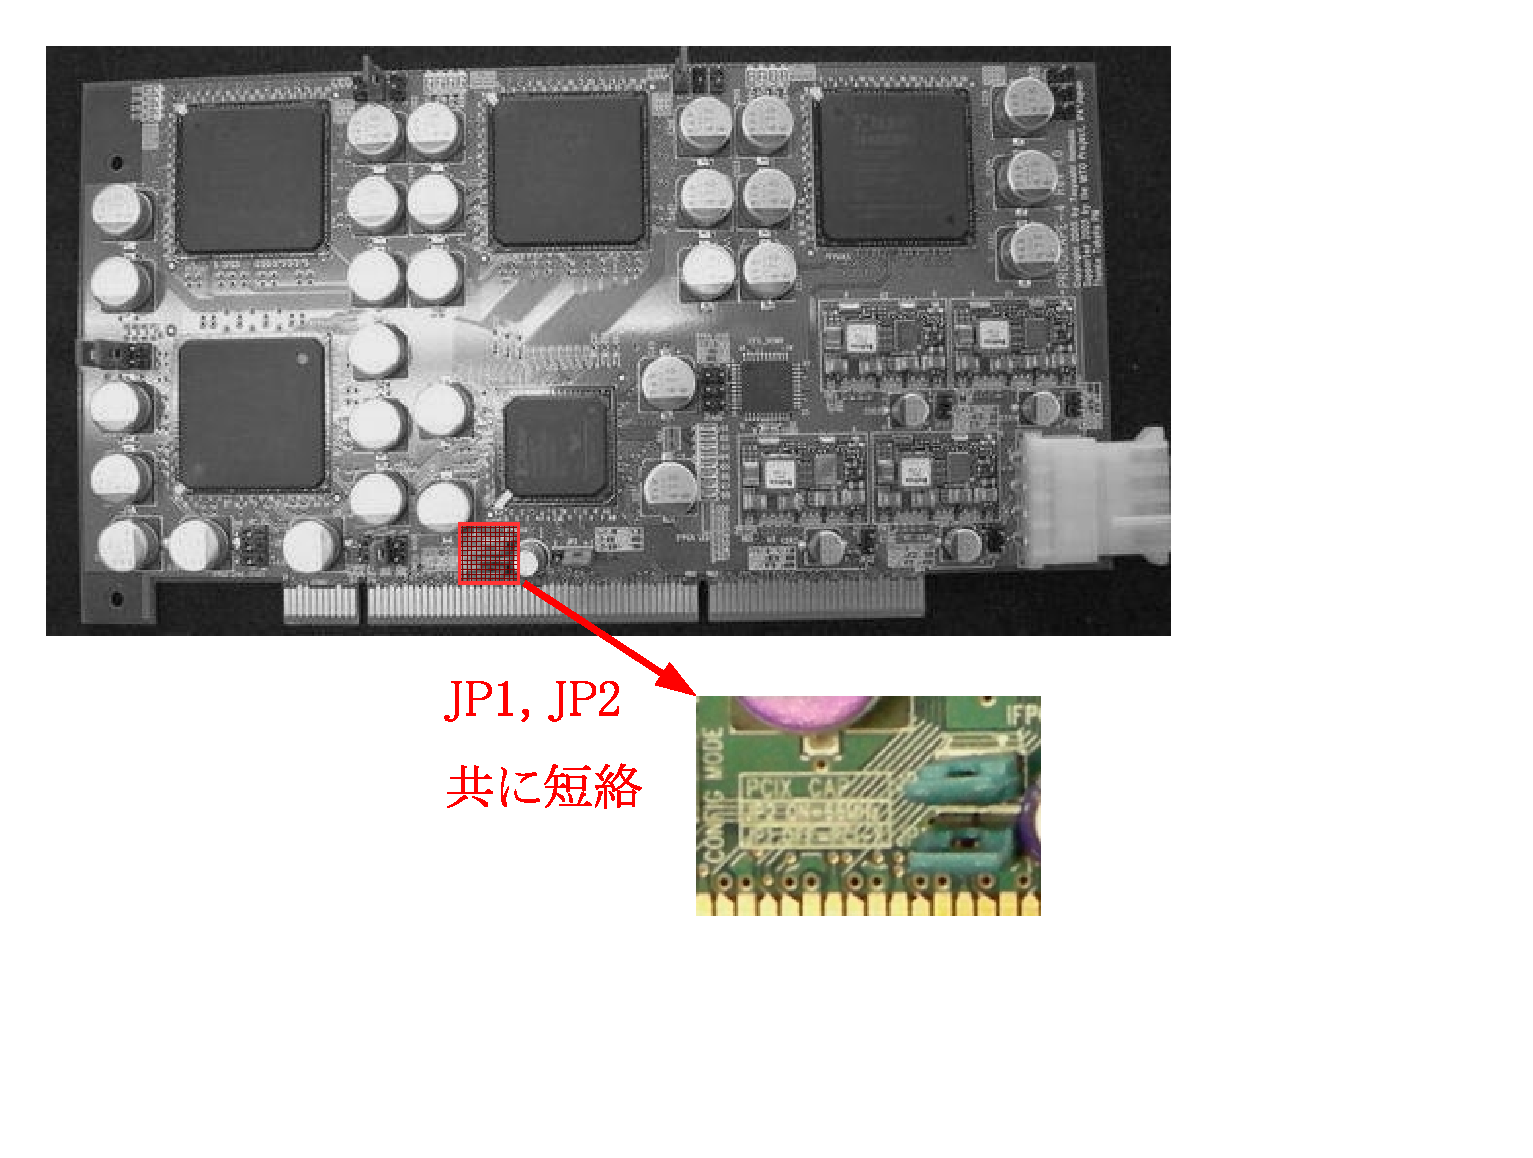
\epsfig{file=fig/pg4-info-jp1jp2,width=100mm}}
\end{minipage}
\caption{JP1, JP2}
\label{fig:Jumper:jp1jp2}
\end{figure}


\begin{figure}[h]
\begin{minipage}[b]{1.0\linewidth}\centering
  \centerline{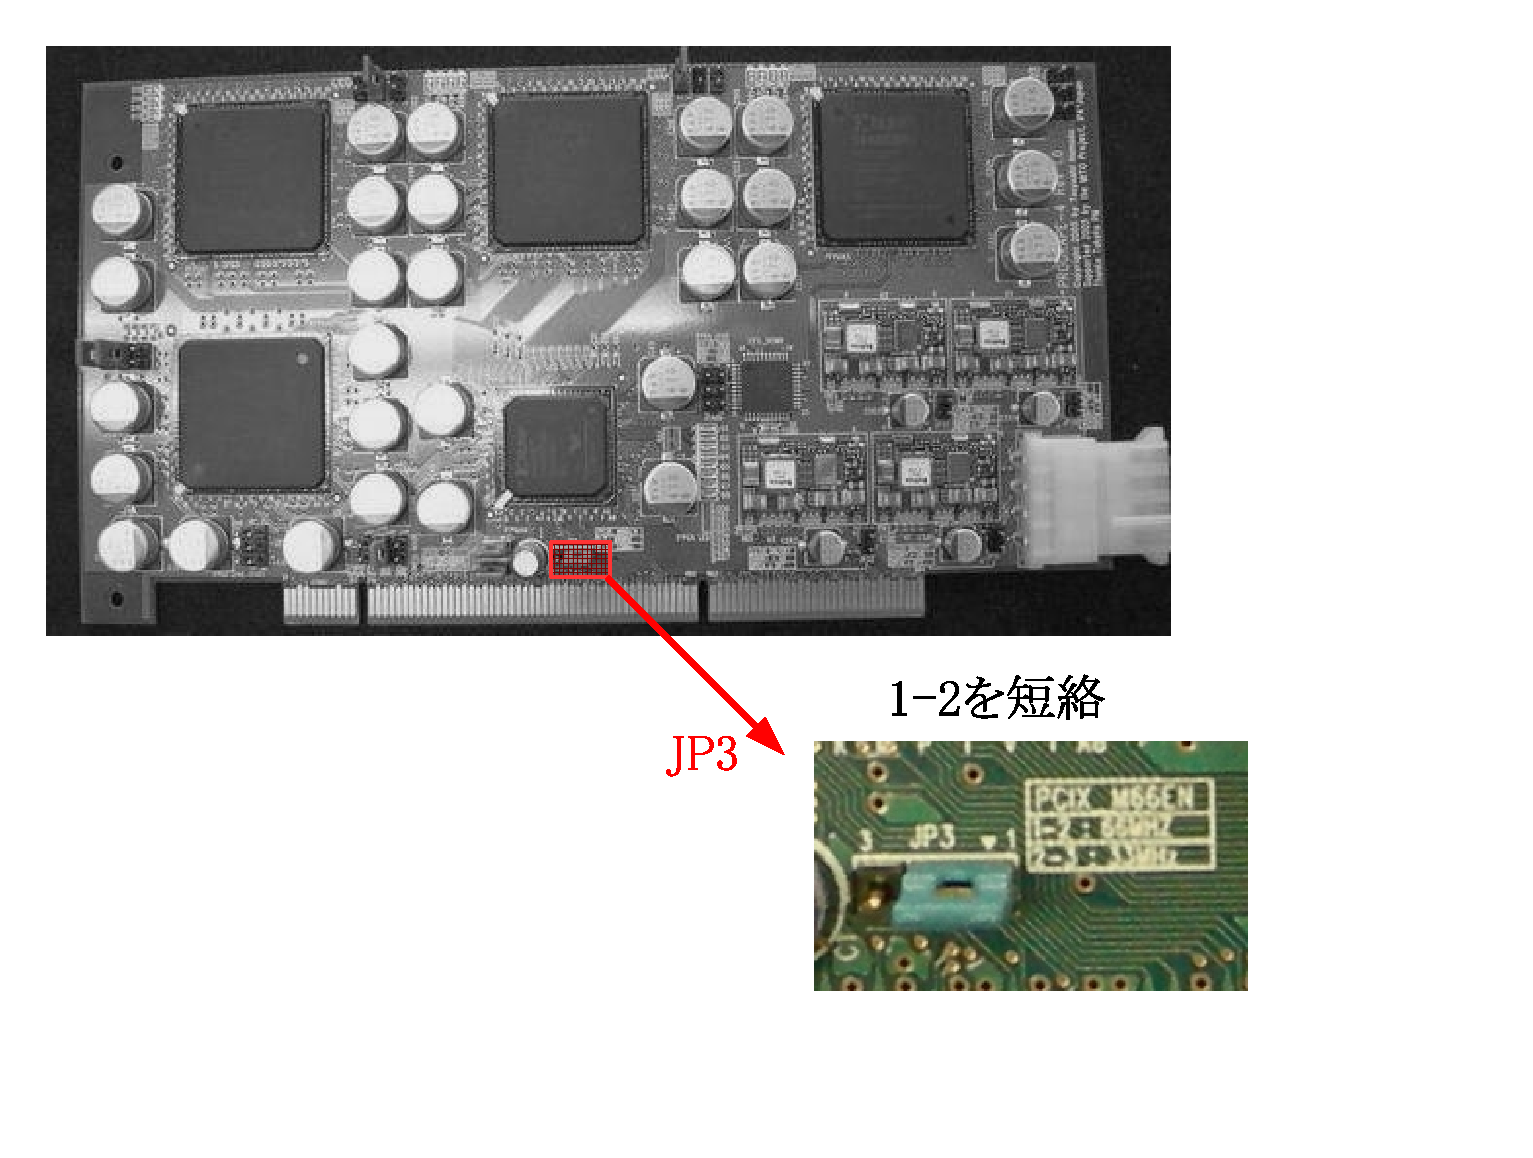
\epsfig{file=fig/pg4-info-jp3,width=100mm}}
\end{minipage}
\caption{JP3}
\label{fig:Jumper:jp3}
\end{figure}

\begin{figure}[h]
\begin{minipage}[b]{1.0\linewidth}\centering
  \centerline{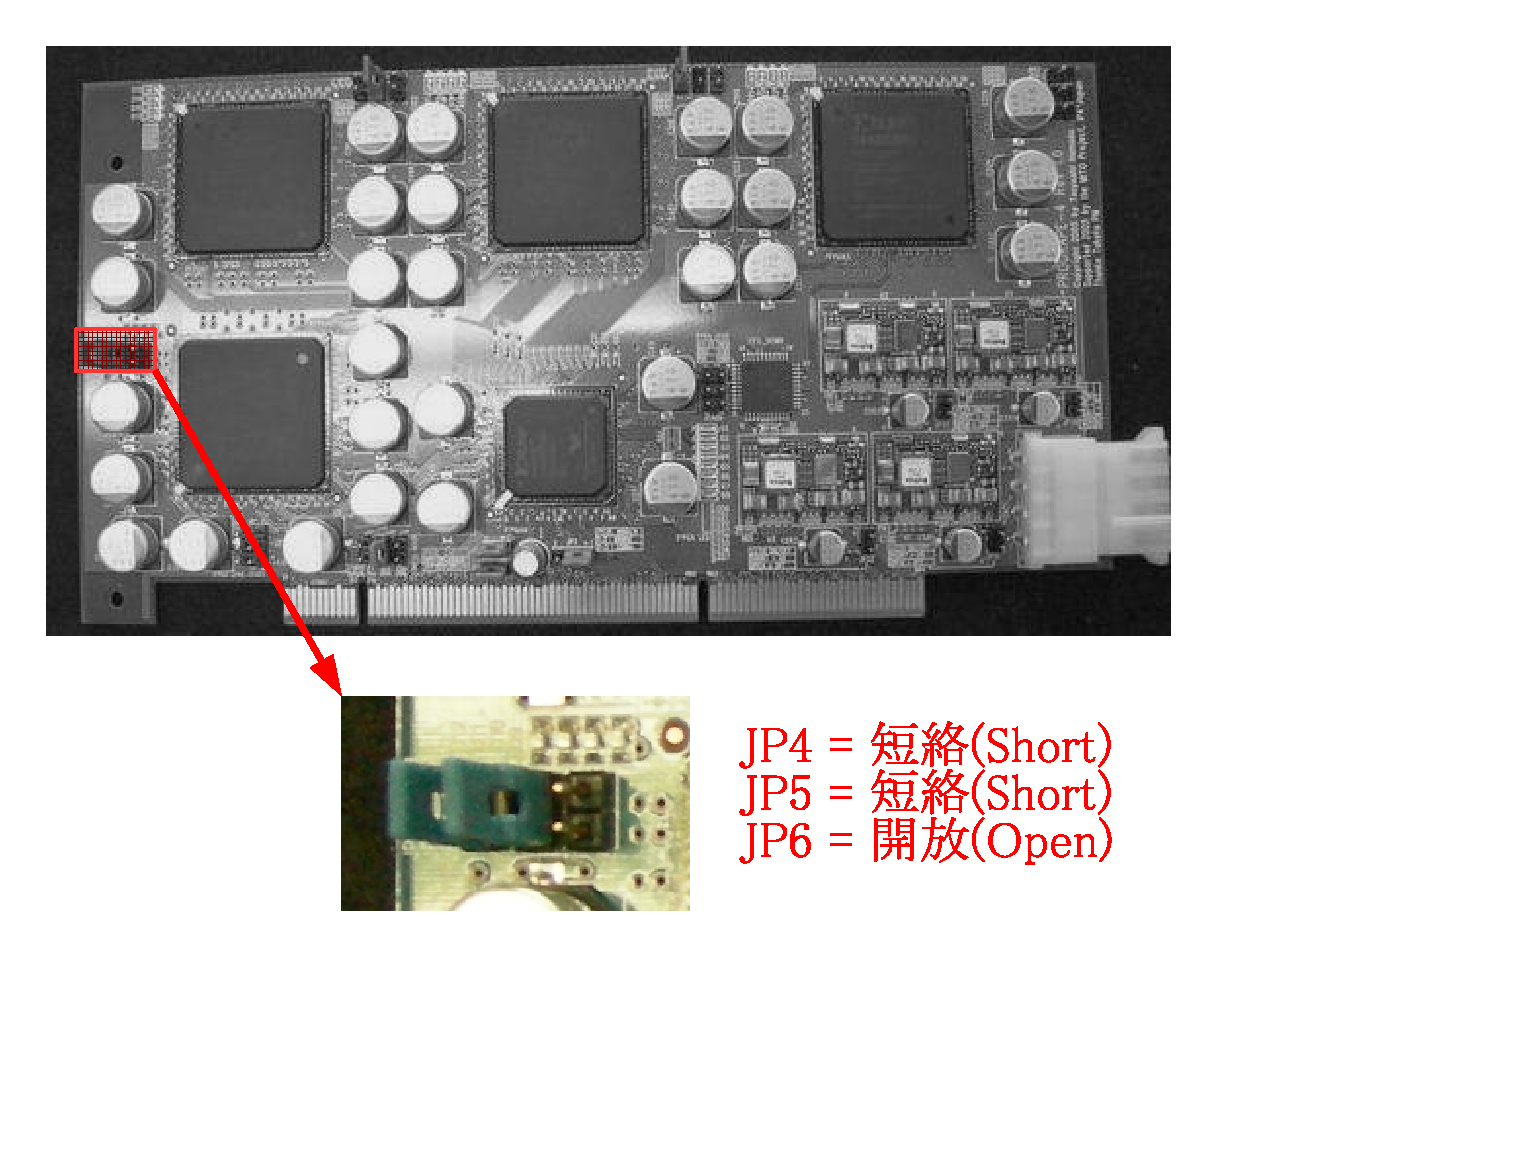
\epsfig{file=fig/pg4-info-jp4jp5jp6,width=100mm}}
\end{minipage}
\caption{JP4,JP5,JP6}
\label{fig:Jumper:jp4jp5jp6}
\end{figure}

\begin{figure}[h]
\begin{minipage}[b]{1.0\linewidth}\centering
  \centerline{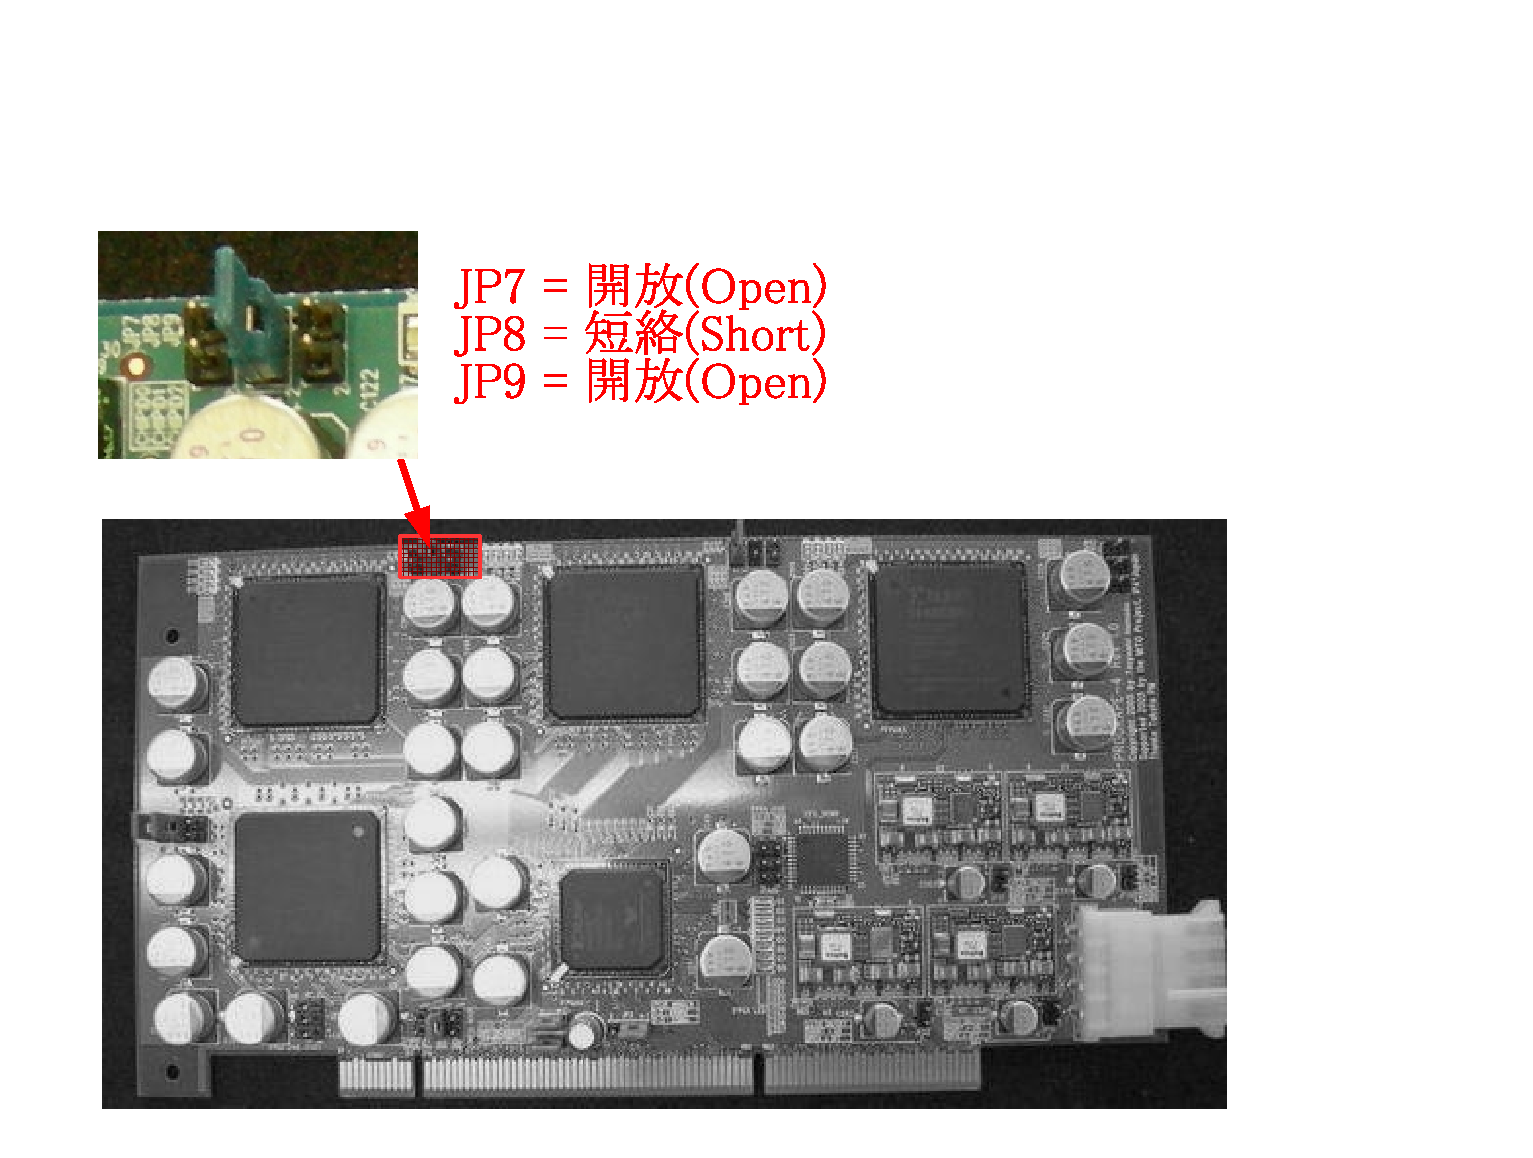
\epsfig{file=fig/pg4-info-jp7jp8jp9,width=100mm}}
\end{minipage}
\caption{JP7,JP8,JP9}
\label{fig:Jumper:jp7jp8jp9}
\end{figure}

\begin{figure}[h]
\begin{minipage}[b]{1.0\linewidth}\centering
  \centerline{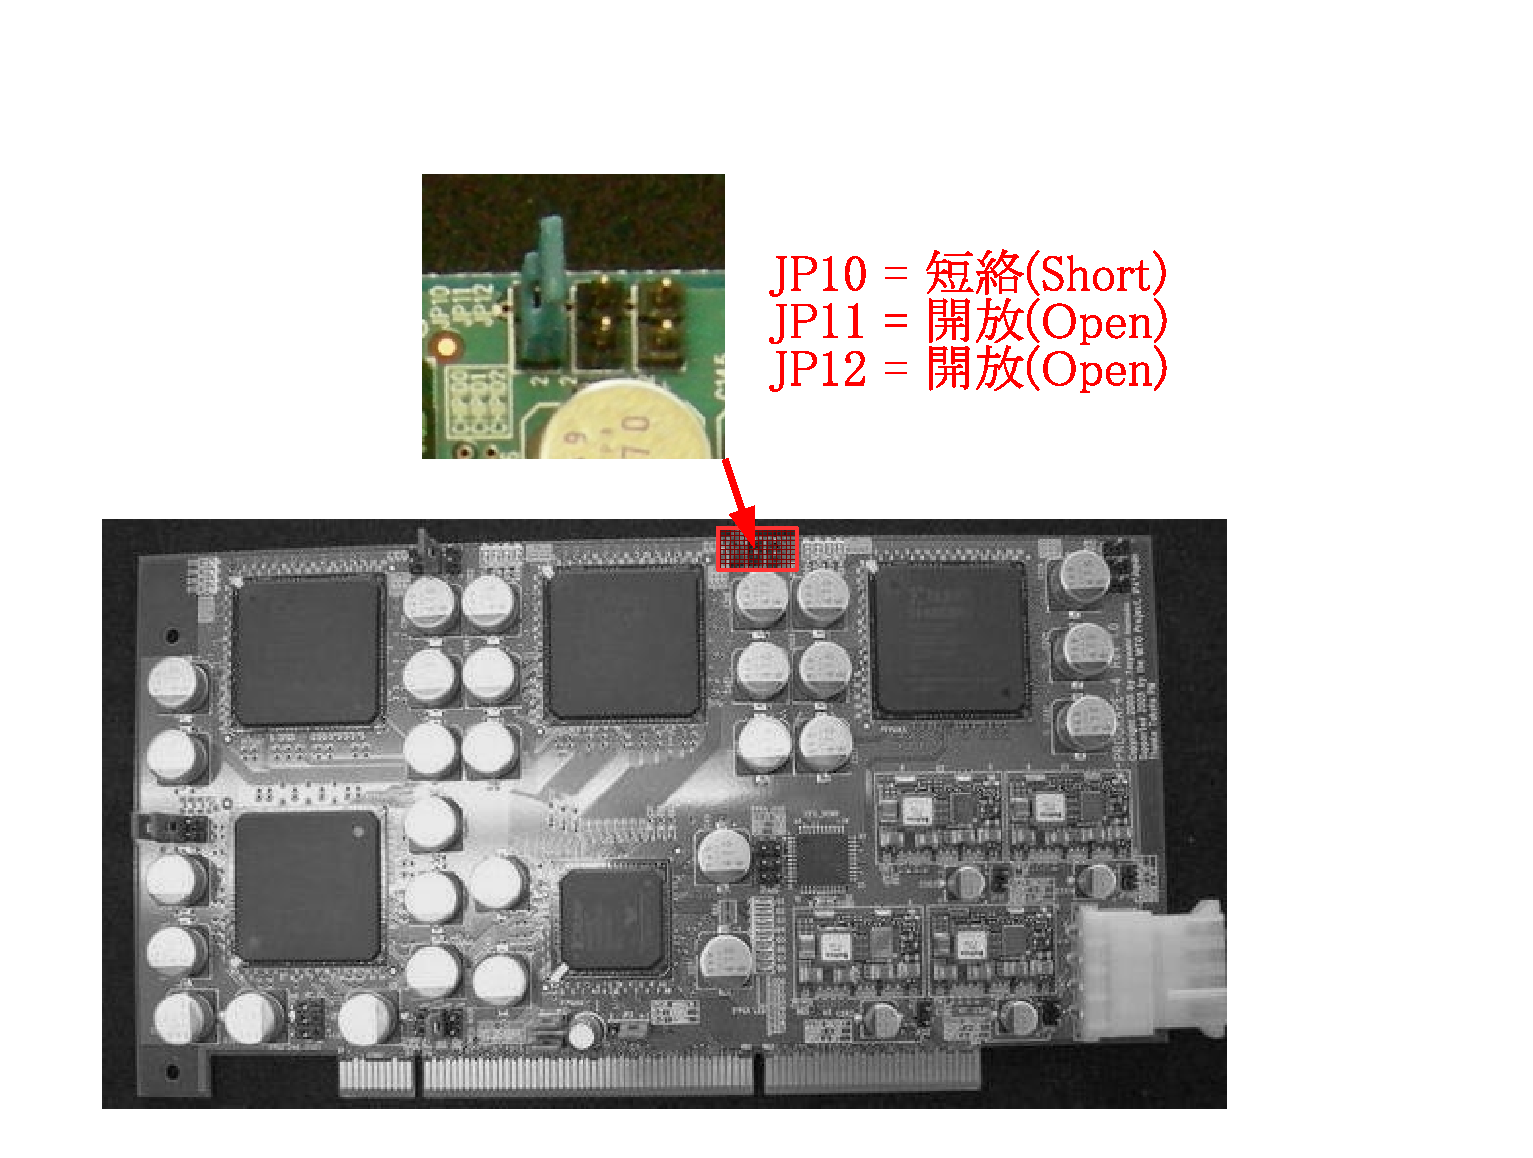
\epsfig{file=fig/pg4-info-jp10jp11jp12,width=100mm}}
\end{minipage}
\caption{JP10,JP11,JP12}
\label{fig:Jumper:jp10jp11jp12}
\end{figure}

\begin{figure}[h]
\begin{minipage}[b]{1.0\linewidth}\centering
  \centerline{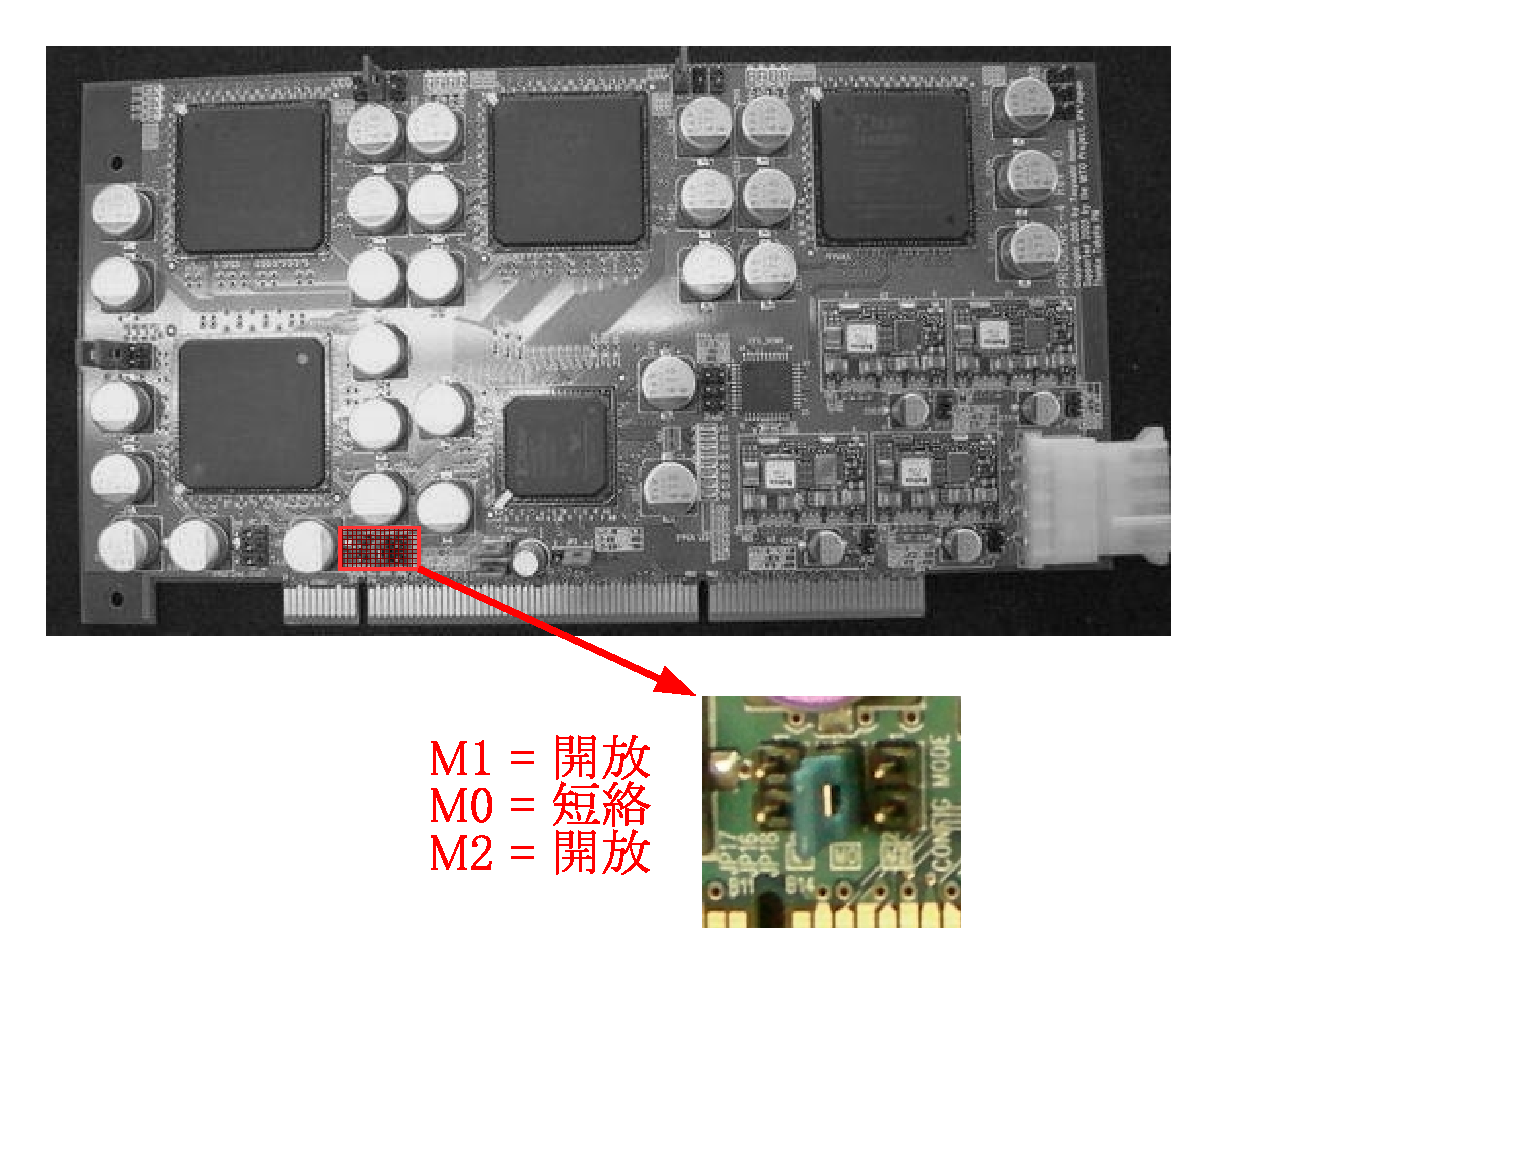
\epsfig{file=fig/pg4-info-m0m1m2,width=100mm}}
\end{minipage}
\caption{M0,M1,M2}
\label{fig:Jumper:m0m1m2}
\end{figure}

�����˼������ʳ��Υ����ѡ������Ƴ���(Open)�ˤ��Ƥ���ޤ���
\footnote{�������Ǥ��������餫�ξ׷�ˤ�ꥸ���Ѥ�����Ƥ��ޤ����Ȥ�
����ޤ������꤬ȯ���������ˤϰ��٥����Ѥ������̤�Ǥ��뤫����ǧ����
����}




\printindex
\end{document}

